\documentclass[12pt]{article}
\usepackage{amssymb} % Para añadir simbolos matematicos
\usepackage{graphicx} % Para añadir imagenes
\usepackage{setspace} % Para modificar espacios entre lineas
\usepackage[left=2.5cm,top=2.5cm,right=2.5cm,bottom=2.5cm]{geometry} % Para establecer el tamaño de los margenes
\author{}
\title{XV Concurso de Programación de la UAM \\ 
"Luis Erick González Moreno" - Solucionario}

\begin{document}
    \maketitle
    \newpage
    \section*{Problema A. Uniendo Puntos}
    \paragraph{}
    \singlespacing
    Este problema consiste en calcular la longitud total, que resulta de sumar las longitudes de las 
    lineas que se forman al unir el punto i con el punto i+1, con $i = 1,2,3,...,n$, y $n$ la cantidad total de puntos,
    hay que tener en cuenta que al llegar al último punto, su siguiente 
    será el primer punto, esta será la ultima longitud que sumaremos. El plano es $\mathbb{R}2$, por lo que cada punto será
    dado con sus respectivas coordenadas ($x, y$). En la imagen se aprecian las distintas lineas que se forman al unir los puntos,
    por lo tanto la respuesta es: \[ longitud_{total} = \sum_{i=1}^{n} l_{i} \] donde $l_{i}$ es la 
    longitud entre el punto $(i)$ e $(i+1)$, esta se puede calcular facilmente con la formula para distancia entre 2 puntos
    \[ \sqrt{(x_{i} - x_{i+1})^2 + (y_{i} - y_{i+1})^2} \]en c++ tenemos una función que nos calcula esto
    la cual es hypot() y recibe como argumentos la diferencia en x y la diferencia en y.
     
    \begin{figure}[h]
        \centering
        \fbox{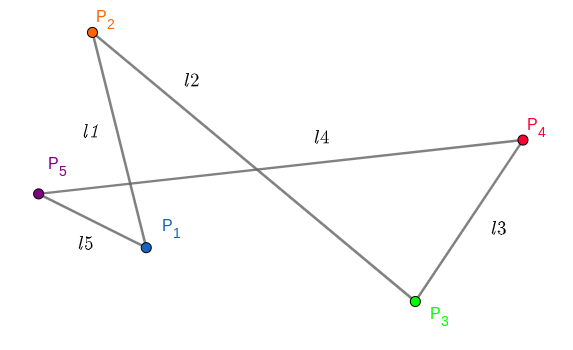
\includegraphics[width=0.6 \textwidth]{problemaA.png}}
        \caption{Puntos caso de ejemplo}
    \end{figure}

    Por último el problema nos pide usar 2
    decimales de precisión, esto se puede lograr en c usando printf("\%.2f",longitud\_total), en c++ si empleamos iostream
    deberemos usar cout $<<$ fixed $<<$ setprecision(2) $<<$ longitud\_total, para usar setprecision() hay que añadir
    en la cabecera a $<$iomanip$>$ y para usar hypot() a $<$cmath$>$.
    \newpage
    \section*{Problema B. Super UAMKid Run}
\end{document}